\subsection{Introducci\'on} En este ejercicio se nos propone implementar un scheduler $Round$-$Robin$ que no permita migraci\'on de procesos (al contrario del $Round$-$Robin$ del ejercicio 4), y cumpliendo una serie de otras caracter\'isticas, como que la asignaci\'on de CPU se realiza al momento que se carga el proceso, y que se elige a la CPU que tiene menor cantidad de procesos activos totales (RUNNING + BLOCKED + READY).

\subsection{Estructura Interna} Para resolver el problema, elegimos la siguiente estructura interna:
\begin{itemize}
	\item \texttt{cant\_cores}: Un n\'umero entero que indica la cantidad de n\'ucleos del procesador.
	\item \texttt{cola\_procesos\_cpu}: Un vector de colas de enteros que guarda, para cada cpu (numeradas del 0 a cant\_cores-1), su correspondiente cola de procesos en el estado de ready.
	\item \texttt{quantum\_original\_cpu}: Un vector de enteros que guarda, para cada cpu, su correspondiente quantum. Notar que esta variable no se modifica nunca, ya que cada cola tiene su quantum fijado desde el inicio de los tiempos.
	\item \texttt{quantum\_restante\_cpu}: Un vector de n\'umeros enteros que contiene, para cada cpu, el quantum restante que le queda al proceso actual que actualmente ejecuta dicha cpu. En cada tick ir\'a decreciendo hasta llegar a 0.
	\item \texttt{cant\_procesos\_cpu}: Un vector de enteros que guarda, para cada cpu, la cantidad de procesos activos totales (RUNNING + BLOCKED + READY).
	\item \texttt{procesos\_por\_nucleo}: Un diccionario de enteros a enteros que establece una relaci\'on entre el pid y la cpu que la ``acogió'', y por lo tanto, a ella le pertenece. El pid es la clave, mientras que el n\'umero de cpu es el significado.
\end{itemize}

Además, la clase cuenta con una función auxiliar, \texttt{int next(int cpu)}, que se encarga de devolver el \emph{pid} del siguiente proceso a ejecutar, removiéndolo de la cola de procesos y reiniciando el \emph{quantum} disponible para el proceso que llega. Notar que en caso de que no hayan procesos en \emph{ready} los últimos dos pasos no se ejecutan y simplemente se devuelve el \emph{pid} de la tarea \emph{idle}.

\subsection{Funcionamiento} Como todo scheduler, la clase posee los siguientes m\'etodos p\'ublicos:
\begin{itemize}
	\item \texttt{SchedRR2(vector<int> argn)}: El constructor de la clase. Se encarga b\'asicamente de inicializar la estructura interna para que tenga sentido (o sea, que se cumpla el invariante de representaci\'on). No encontramos nada importante a destacar en este m\'etodo m\'as que aclarar que el vector \emph{cant\_procesos\_cpu} se llena con ceros ya que al inicio todas las cpu tienen 0 procesos activos totales, y que el vector \emph{cola\_procesos\_cpu} se llena con colas de enteros vac\'ias.
	\item \texttt{void load(int pid)}: Se encarga de cargar el proceso identificado por el pid recibido por par\'ametro. Pueden haber dos escenarios en la carga de un proceso:
	\begin{enumerate}
		\item Que sea un nuevo proceso que se est\'e cargando, en cuyo caso se debe elegir una de las cpu's que tienen menor cantidad de procesos activos totales para que ``apadrine'' a este nuevo proceso entrante, sumarle 1 a la cantidad de procesos de \'esa cpu, agregar ese proceso a la cola de procesos de \'esa cpu, y por \'ultimo agregar la relaci\'on pid-cpu en el diccionario \emph{procesos\_por\_nucleo}.
		\item Que sea un proceso existente que se acaba de desbloquear, en cuyo caso se debe obtener la cpu a la cual pertenece este proceso y agregarlo a la cola de procesos de la misma.
	\end{enumerate}
	\item \texttt{void unblock(int pid)}: Se vuelve a cargar la tarea que dej\'o de estar bloqueada, lo que consiste simplemente en llamar a la funci\'on \texttt{load}.
	\item \texttt{int tick(int cpu, const enum Motivo m)}: Esta funci\'on se divide en tres casos dependiendo de qu\'e ocurri\'o en el \'ultimo tick ejecutado por la cpu:
	\begin{enumerate}
		\item TICK: En el caso de que haya ejecutado un tick entero, pueden ocurrir dos cosas: 1) Us\'o todo su quantum; 2) No us\'o todo su quantum. En el caso 1 hay que encolar el proceso actual y traer al siguiente proceso a la cpu invocando a la funci\'on \texttt{next(cpu)}. En el caso 2 s\'olo hay que restarle 1 al quantum restante de la cpu y devolver el pid de la tarea actual, ya que es a la que le toca seguir ejecutando.
		\item BLOCK: En el caso de que la tarea se haya bloqueado s\'olo hay que llamar a la funci\'on \texttt{next(cpu)} explicada en la secci\'on ``Estructura Interna''.
		\item EXIT: En el caso de que la tarea haya finalizado, hay que restarle 1 a la variable que guarda la cantidad de procesos activos totales de cada cpu (ya que ahora este proceso no forma parte de los procesos activos totales de la cpu), borrar del diccionario el pid del proceso que acaba de finalizar e invocar a la funci\'on \texttt{next(cpu)} para cargar un nuevo proceso a la cpu.
	\end{enumerate}
	Si por alg\'un error misterioso el motivo no es ninguno de los descriptos anteriormente, se proceder\'a a enviar un mensaje de error por el standard error.
\end{itemize}

\subsection{Comparación entre SchedRR y SchedRR2}

%waiting time empeora con migracion de procesos xq hay un tiempo de cambio de procesador que es tiempo muerto.

%para las tareas muy interactivas que requieran bloquearse 


%HAY QUE HACER TODA LA PARTE IMPORTANTE, O SEA EXPLICAR EN QUE CASOS ESTA BUENO  MIGRACION DE PROCESOS Y EN QUE CASOS NO, Y DAR LOTES Y GRAFICAR Y MOSTRAR LAS METRICAS QUE MEJORAN O EMPEORAN EN CADA CASO.

%con migracion se desperdicia menos cpu.
%con migracion aumenta el waiting time por el cambio de cpu.


%estaria bueno ver que pasa cuando las tareas entran en algun momento especifico.
A continuación analizamos algunas de las ventajas y desventajas de tener migración de procesos entre las CPUs y no tenerlo.

En las figuras \ref{fig:ej8-1} y \ref{fig:ej8-2} contrastamos la eficiencia entre ambas políticas de \emph{scheduling}.

\begin{figure}[H]
  \centering
  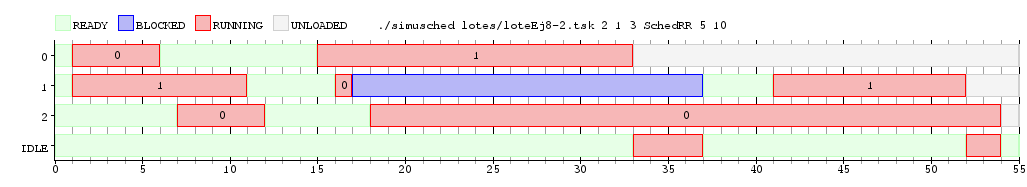
\includegraphics[width=1\textwidth]{img/imgEj8-1}
  \caption{}
  \label{fig:ej8-1}
\end{figure}



\begin{figure}[H]
  \centering
  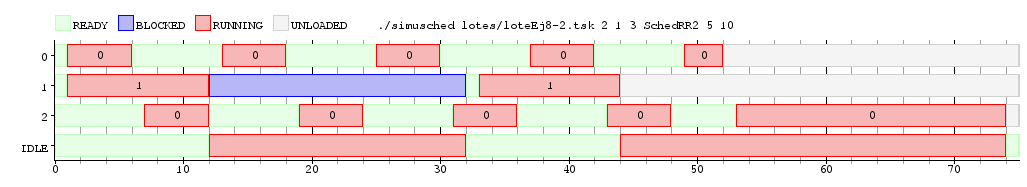
\includegraphics[width=1\textwidth]{img/imgEj8-2}
  \caption{}
  \label{fig:ej8-2}
\end{figure}

En estas figuras observamos que el tener migración reduce el desperdio de cpu, ya que en el tiempo en que el proceso 1 se bloquea en el \texttt{SchedRR2}(que no tiene migración) ese tiempo de procesamiento se pierde. Esto se muestra en el hecho de que el tiempo en que el proceso \emph{idle} corre es mayor \texttt{SchedRR2} que en el \texttt{SchedRR}.

En las figuras \ref{fig:ej8-3} y \ref{fig:ej8-4} por otra parte vemos que, aunque el no tener migración de procesos potencialmente desperdicia más los procesadores, si se realizan demasiadas migraciones esto resulta en un tiempo de ejecución global peor.

\begin{figure}[H]
  \centering
  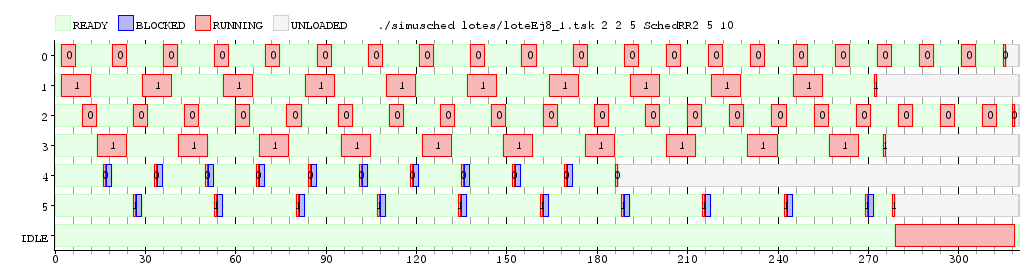
\includegraphics[width=1\textwidth]{img/imgEj8-3}
  \caption{}
  \label{fig:ej8-3}
\end{figure}



\begin{figure}[H]
  \centering
  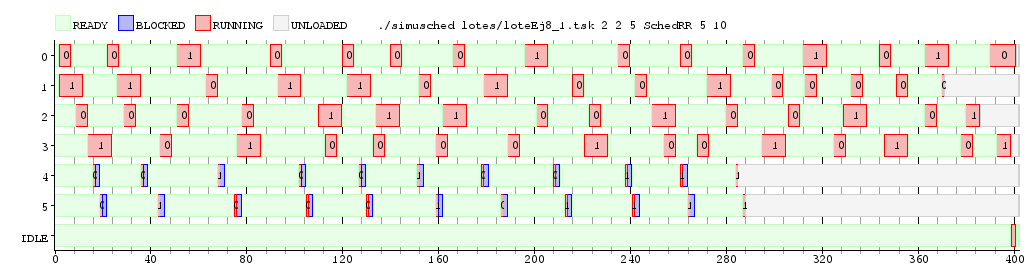
\includegraphics[width=1\textwidth]{img/imgEj8-4}
  \caption{}
  \label{fig:ej8-4}
\end{figure}











